\chapter{Introduction}
\label{chap:intro}

\section{Galaxy Evolution}
\label{sec:gal_evolution}

\section{Galaxy properties}
\label{sec:gal_properties}

\subsection{Color}
\label{sec:color}

\begin{figure}[!ht]
  \centering
  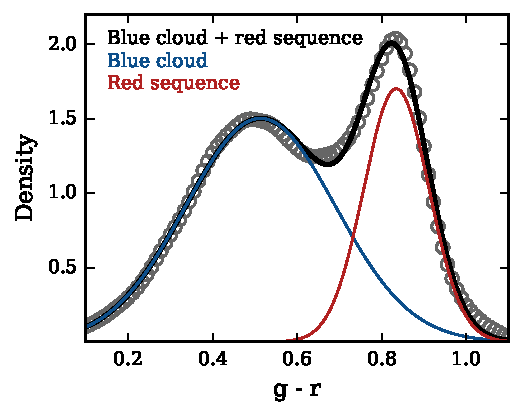
\includegraphics[width=0.8\textwidth]{gr_dist.pdf}
  \caption{$g-r$ colour distributions for low-redshift galaxies in
    SDSS groups.  Circles correspond to the smoothed density
    distribution of the data, the black line shows a double-Gaussian
    fit, and the red and blue lines show the components of the
    double-Gaussian fit corresponding to the red sequence and the blue
  cloud.}
  \label{fig:gr_dist}
\end{figure}

Color is one of the simplest measures with which one can characterize
the properties of a galaxy.  The color of a galaxy is defined as the
difference between the magnitudes of a galaxy in two different bands.
As an example, the $g - r$ colour for a SDSS galaxy would be the
difference between the galaxy's $g$-band magnitude (centred on
$477.0\,\mathrm{nm}$) and $r$-band magnitude (centred on
$623.1\,\mathrm{nm}$).  Many studies have shown the colour
distributions of galaxy populations to be well fit by a
double-Gaussian across many environments \citep{balogh2004,
  baldry2006}.  The two
components of the double-Gaussian fit are referred to as the `red
sequence' and the `blue cloud'.  In Fig.~\ref{fig:gr_dist} I show the
$g-r$ colour distribution for a sample of low-redshift ($z < 0.05$)
SDSS group galaxies, and a double-Gaussian fit (black) as well as the
two components corresponding to the blue cloud and the red sequence.
The red sequence peaks at red colours and has a
relatively small dispersion, whereas the blue cloud is a bluer and
broader sub-population.
\par
The overlap region between the red sequence
and the blue cloud is known as the ``green valley'' and is thought to
be a transition region.  It has been hypothesized that galaxies evolve
from the blue cloud, through the green valley, onto the red sequence
over time \citep[e.g.][]{trayford2016}.  An important piece of evidence in
support of
this evolutionary scenario is the Butcher-Oemler (BO) effect.  The BO
effect is an observed positive correlation between the fraction of blue
galaxies within galaxy clusters and redshift, first observed by
\citet{butcher1978} and subsequently observed by many more recent
studies \citep[e.g.][]{butcher1984, ellingson2001, loh2008,
  urquhart2010}.  Therefore it seems that at early times populations
of galaxies in clusters were bluer than they are at present day.
\par
In addition to redshift correlations, galaxy colours also depend
strongly on stellar mass.  Both the fraction of red galaxies \citep{baldry2006,
  bamford2009, kimm2009, prescott2011} as well as the average colour
of galaxies \citep{cooper2008, vandenbosch2008a} increase significantly toward
high stellar masses.  These stellar mass trends are not only in place
in the local Universe, but also at high redshift \citep{grutzbauch2011}.

\subsection{Morphology}
\label{sec:morph}

\begin{figure}[!ht]
  \centering
  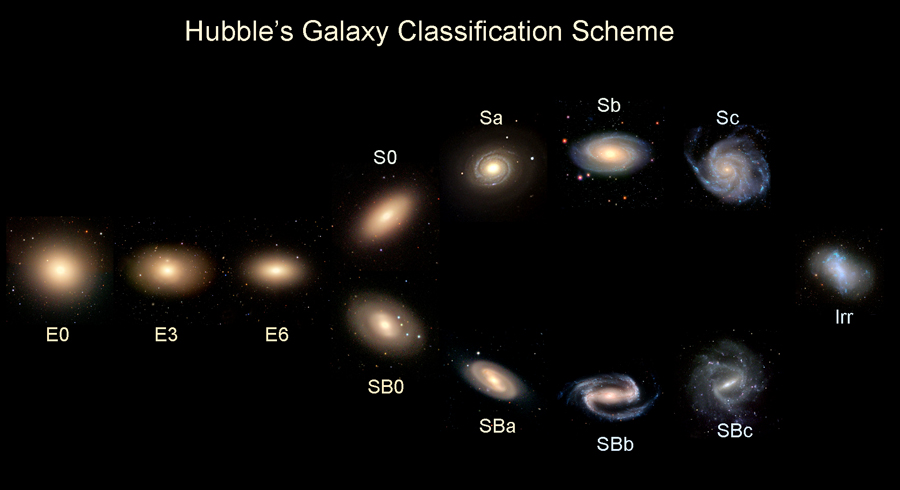
\includegraphics[width=\textwidth]{tuning_fork.jpg}
  \caption{The Hubble tuning fork classification diagram.  Image
    credit: Galaxy Zoo.}
  \label{fig:tuning_fork}
\end{figure}

The first robust classification scheme for galaxies was laid out by
\citet{hubble1926}.  This classification scheme (see
Fig.~\ref{fig:tuning_fork}), which has since become known colloquially
as Hubble's tuning fork diagram, broadly divides the galaxy
population into elliptical and spiral galaxies.  The class of
ellipticals is further sub-divided by ellipticity, $e = 0,1,2,...,7$,
where $e = 10 \times (a-b)/a$, with $a$ and $b$ denoting the major and
minor axis of the ellipse, respectively.  Ellipticals can then be
classified as E$e$, where E$0$ would be perfectly round (in
projection) and E$7$ would be a highly elongated ellipse.  Spiral
galaxies are sub-classified by the brightness of the central region as
well as how tightly coiled are their spiral arms.  Spirals denoted as
S$a$ are galaxies with bright central bulges and tightly wound spiral
arms, galaxies denoted as S$c$ are galaxies with weak bulges and
loosely wound spiral arms, and S$b$ spirals represent an intermediate
class between the two.  Spirals are also divided by the presence of a
bar, or lackthereof, with barred spirals being denoted as SB galaxies.
S$0$ or lenticular galaxies appear to have structure intermediate
between ellipticals and spirals are characterized by a strong bulge
region, as well as the presence of a disc devoid of spiral arms.
Following the nomenclature used by Hubble, it is commonplace to refer
to elliptical and S0 galaxies as ``early-types'' and spiral galaxies
as ``late-types'', due to their positions on the tuning fork diagram.
It is however important to note that this nomenclature refers solely
to the position on the diagram and is agnostic to evolutionary
theories\footnote{Though not always given credit, Hubble was
  very clear on this point stating that the classification was made
  ``without prejudice to theories of evolution'', and that ``temporal
  connotations are made at one's peril''}.
\par
The first technique used to determine galaxy morphologies was visual
classifications \textbf{(REF)}.  Visual classifications are able to
accurately divide galaxy samples into spirals, ellipticals, or S0's,
however the time consuming nature of this practice has historically
made it difficult to apply to large data sets.  That being said, the
onset of citizen science programs such as the Galaxy
Zoo\footnote{https://www.galaxyzoo.org} \citep{lintott2008} have made
the application of visual classifications to large data sets
increasingly feasible.
\par
Modern automated techniques often rely on photometric measurements of 
light profiles of a galaxies to classify morphology.  In particular, two
main measures known as the single \ser index ($n$), and the
bulge-to-total ratio ($B/T$) are commonly used to quantitatively determine
the morphology of a galaxy.
\par
The \ser index, $n$, is a free parameter of the so-called
\ser profile \citep{sersic1968} which often fit to galaxy
intensity profiles.  Using the \ser profile, the intensity of a
galaxy as a function of radius is given by 

\begin{equation}
  I(r) = I_e \exp \{-k [(r/r_e)^{1/n} - 1]\},
\end{equation}

\noindent
where $r_e$ is the effective radius which encloses half of the total
light, $I_e$ is the intensity at the effective radius, and $k$ is a
normalization factor which depends on the S{\'e}rsic index $n$.  In
general, the S{\'e}rsic index runs between $1 \le n \le 8$.  Disc
dominated, spiral galaxies have light profiles which are well fit by a
\ser index of $n \lesssim 2$, with the special case of a purely
exponential disc being given by $n=1$.  Elliptical galaxies have more
centrally concentrated light profiles, and are therefore well fit by
larger \ser indices, $n \gtrsim 2$.  A commonly used empirical law to
describe the brightness profiles of elliptical galaxies is de
Vaucouleurs' law which states that the intensity of an elliptical
galaxies goes as $\log I(r) \propto r^{1/4}$, and this is also just a
special case of the \ser profile with $n=4$.
\par
Instead of modelling the light profile a galaxies as a single
component, bulge + disc decompositions are often used as another
method of classifying the morphology of galaxies.  In this scenario
the light profile of the bulge and disc are modelled separately, it is
common to model the bulge with an $n=4$ de Vaucouleurs profile and the
disc with an $n=1$ exponential profile \citep[e.g.][]{simard2002}, the
sum of these two
components is then the model for the galaxy as a whole.  The fraction
of the total light produced in the bulge component is the bulge-to-total ratio
($B/T$) which is used as a morphological discriminator for galaxies.
Pure elliptical galaxies will have $B/T \to 1$, and pure disc galaxies
will have $B/T \to 0$.
\par
Galaxy morphology is also strongly correlated with stellar mass, with
high-mass galaxies showing earlier types morphologies.  This trend has
been confirmed using different probes of morphology, such as
S{\'e}rsic index \citep{vanderwel2008}, bulge-to-total ratio
\citep{bluck2014}, as well as visual morphological classifications
\citep{bamford2009}.  

\subsection{Star formation rates}
\label{sec:sfr}

\begin{figure}[!ht]
  \centering
  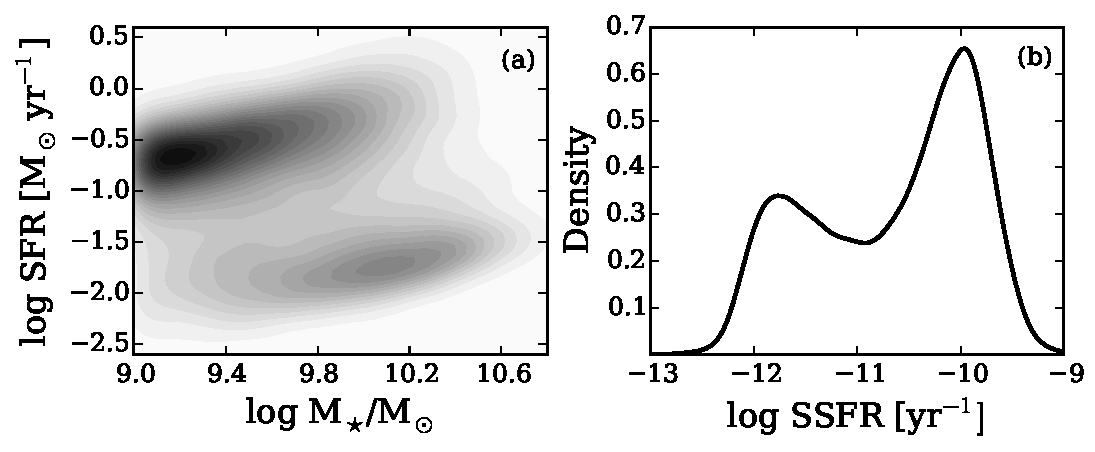
\includegraphics[width=\textwidth]{m_sfr.pdf}
  \caption{Left: Star formation rate versus stellar mass for a sample
    of low-redshift SDSS group galaxies.  Right: Specific star
    formation rate density distribution for a sample of low-redshift
    SDSS group galaxies.}
  \label{fig:m_sfr}
\end{figure}

The star formation rate (SFR) of a galaxy is defined intuitively as the rate
at which a galaxy generates new mass in the form of stars, measured in
units of solar-masses per year ($\Msun\,\mathrm{yr^{-1}}$).  Being
able to accurately determine the SFRs of galaxies is crucial for the
study of galaxy evolution.  Currently there are multiple methods used
to derive SFRs for galaxies, each relying on different aspects of
galactic electromagnetic emission.
\par
One of the most common methods is to derive SFRs from UV or IR
continuum 
emission using conversion factors.  UV continuum emission directly
probes light emitted from young stars and therefore is a strong
indicator of a galaxies SFR.  The largest shortcoming of UV emission
is the fact that the existance of large amounts of interstellar dust
causes galaxies to be relatively opaque to UV photons.  In fact,
approximately half the emission from stars in the Universe is absorbed
and re-emitted by dust in the infrared \citep{kennicutt2012}.
The leads to IR continuum emission from dust being a useful probe of
galaxy SFRs.  As mentioned previously, both UV and IR continuum
luminosities can be converted to SFRs using wavelength-dependent
conversion factors.
\par
In addition to continuum emission, emission line strengths can also be
used as star formation indicators, with the $\mathrm{H}\alpha$ line
being the most commonly used emission line indicator for galaxies in
the local Universe.  As before, using the correct conversion factor
one can determine a SFR estimate from $\mathrm{H}\alpha$ emission, and
similar to the UV continuum, the largest decrement to this method is
dust attenuation.  \citet{kennicutt2012} provide a compilation of up
to date SFR conversion factors for both continuum and line emission,
across a wide range in wavelength.
\par
Another common star formation indicator is the 4000 angstrom break
($\mathrm{D_n}4000$), which refers to the strength of the break at
$4000\,\mathrm{\mathring{A}}$ in a galaxy's spectrum.  Galaxies with
old stellar populations and little recent star formation will show a
strong $\mathrm{D_n}4000$ break due to strong metal absorption in the
atmospheres of old stars as well as a lack of UV emission from young,
hot stars \citep{hamilton1985}.  Galaxies with strong recent star
formation will show a correspondingly small break at
$4000\,\mathrm{\mathring{A}}$.
\par
\textbf{SED fitting...}
\par
Across a wide range of environments galaxies
can be divided into two main subpopulations based on their SFRs, those
galaxies which are actively forming stars and those quiescent galaxies
whose star formation has ceased \citep{wetzel2012}.  One way to
define the population of star-forming galaxies is to use the
``star-forming main sequence'' (SFMS).  The SFMS is a tight
correlation between SFR and stellar mass located in the upper region
of $\mathrm{SFR} - M_\star$ plane.  The SFMS for low-redshift galaxies
in SDSS groups is easily visible in Fig.~\ref{fig:m_sfr}(a) ranging
between $\sim -1 < \log \mathrm{SFR} < 0$.  Due to the correlation
between SFR and stellar mass, it is useful to normalize SFR by galaxy
stellar mass, known as the specific star formation rate
($\mathrm{SSFR} = \mathrm{SFR}/M_\star$).  Like the distribution of
galaxy color, the SSFR distribution for galaxy populations is also
bimodal (see Fig.~\ref{fig:m_sfr}(b)).  This bimodality in SSFR
provides another method for distinguishing between star-forming and
passive galaxies.  Recent observations have shown that across
many environments in the local Universe, the division between
the active and quiescent populations (ie.\ the local minimum in the
SSFR distribution) is found at $\log \mathrm{SSFR} \simeq -11$
\citep{wetzel2012}.

\begin{figure}[!ht]
  \centering
  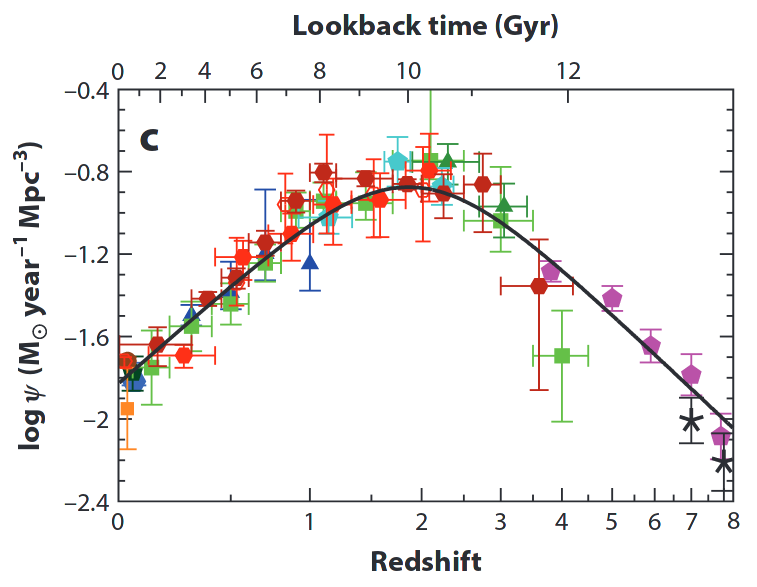
\includegraphics[width=0.8\textwidth]{lilly_madau.png}
  \caption{Cosmic star formation rate density as a function of
    redshift, using both IR and UV derived SFRs.  Image credit:
    \citet{madau2014}.}
  \label{fig:lilly_madau}
\end{figure}

Star formation activity has also been shown to depend on redshift.
The normalization of the SFMS shifts to larger SFRs with increasing
redshift \citep{karim2011, whitaker2012, lee2015, erfanianfar2016},
star-forming fractions of galaxies in groups and clusters (at a given
stellar mass) increase with redshift \citep{mcgee2011, hou2013,
  nantais2013}, as well the average SSFRs of galaxies increase with
redshift as $(1+z)^\alpha$ where $\alpha \sim 2-4$
\citep{oliver2010, whitaker2012}, at least out to $z=2$.  On larger
scales, the density of star formation rate in the Universe has been
shown to have been decreasing to the present day from its peak at $z
\simeq 2$ \citep[e.g.][]{madau1998, madau2014}.
Fig.~\ref{fig:lilly_madau} shows this in the form of an updated
version of the famous Lilly-Madau plot taken from \citet{madau2014}.

\section{Galaxy groups}
\label{sec:groups}

\begin{figure}[!ht]
  \centering
  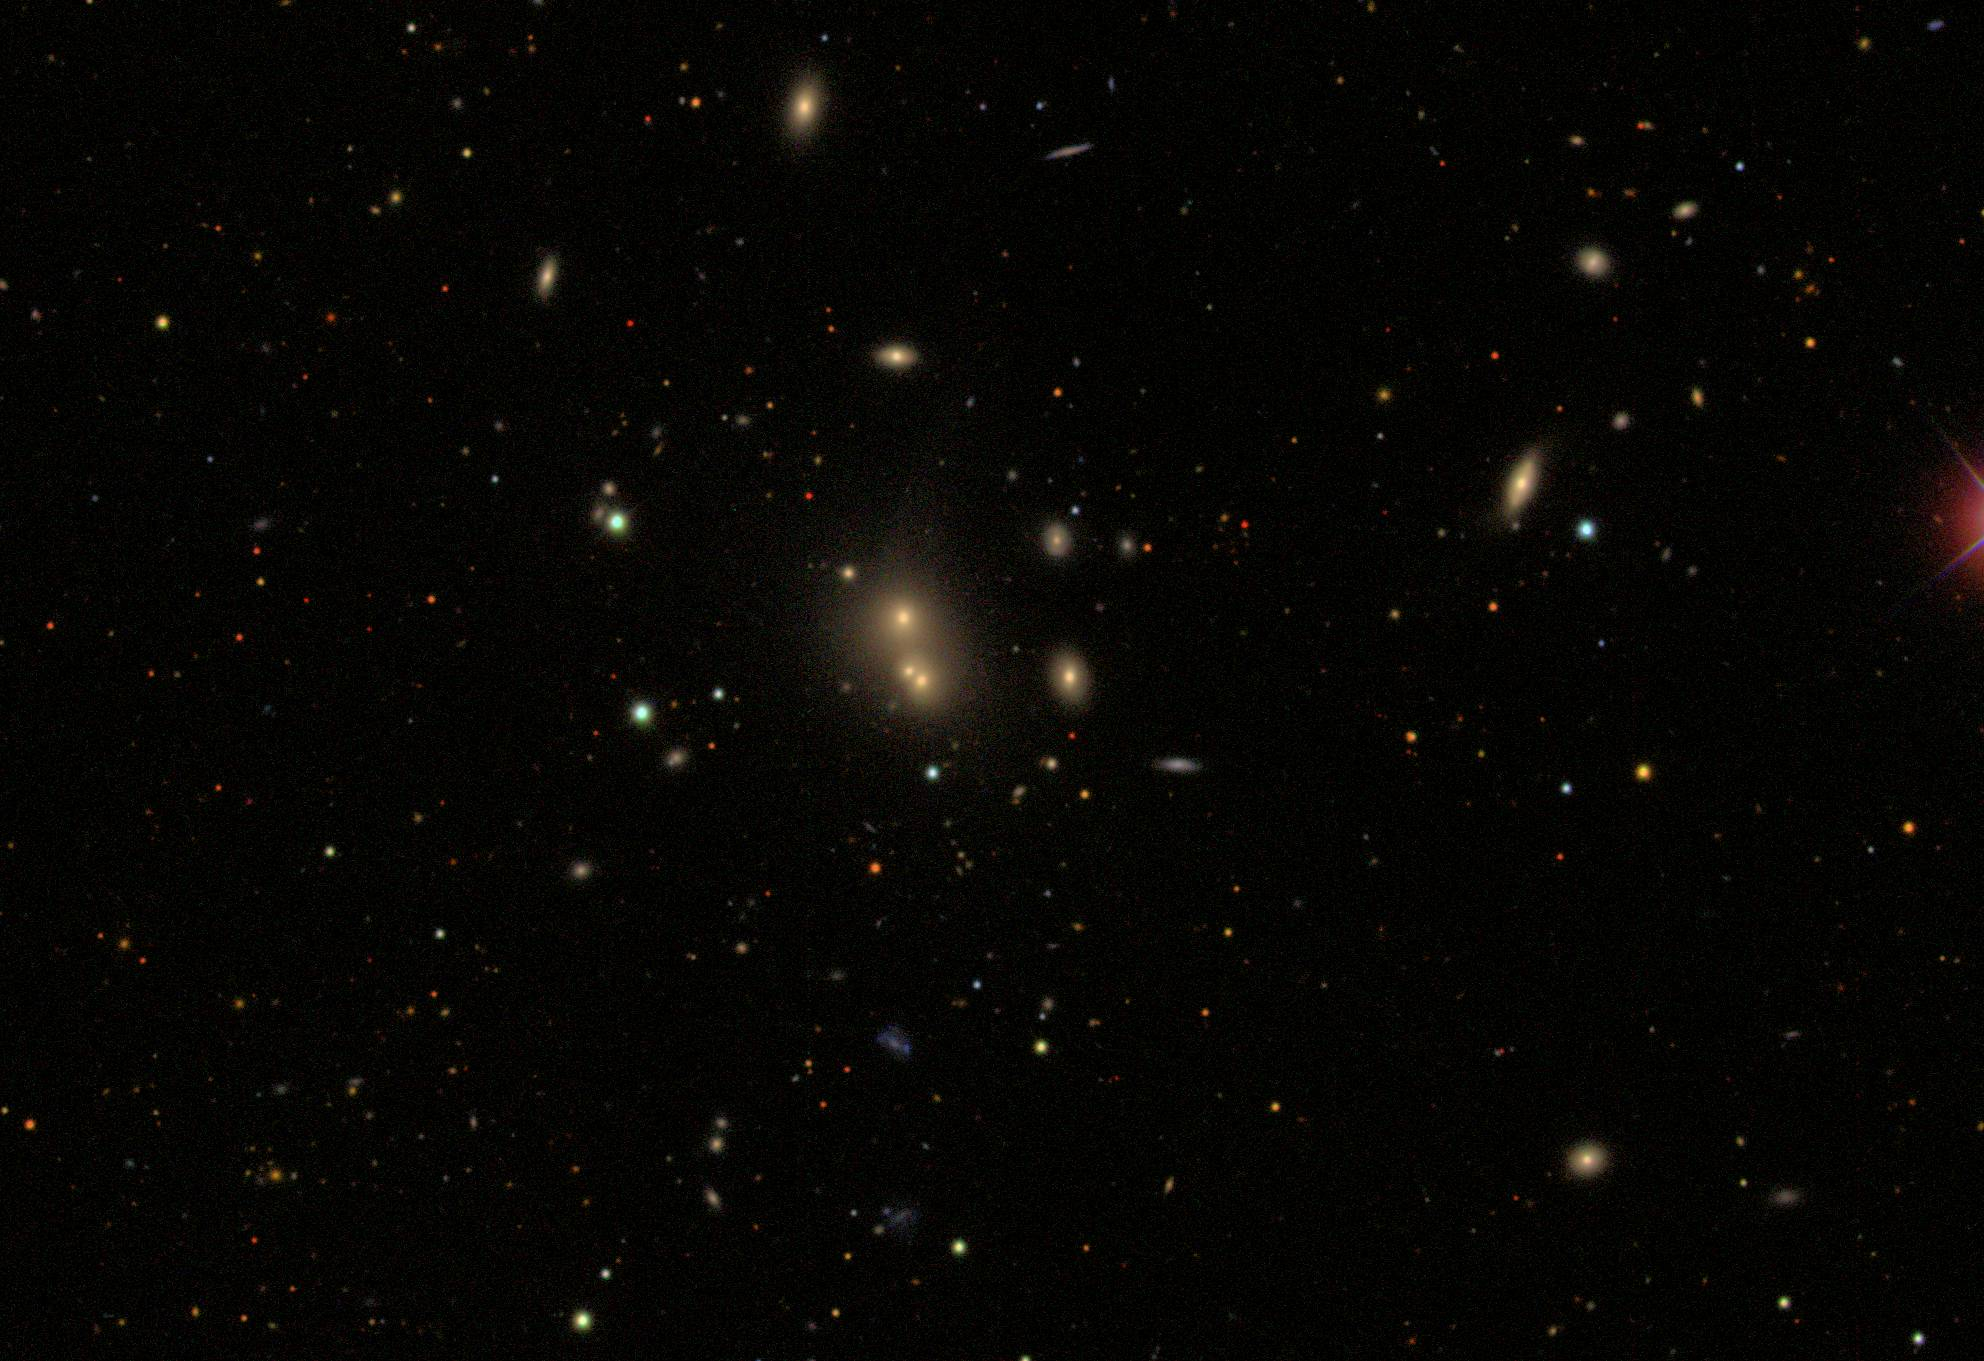
\includegraphics[width=0.8\textwidth]{225.jpeg}
  \caption{SDSS image of a galaxy group from the \citet{yang2007}
    group catalogue.  Image credit: Sloan Digital Sky Survey.}
  \label{fig:sdss_225}
\end{figure}

Galaxy groups are the most commonly populated environment in the local
Universe \citep{geller1983, eke2005}, and also are a regime in which
many processes capable of driving galaxy evolution are efficient.
While populations of galaxies in the isolated field and large clusters are
dominated by active, late-type and passive, early-type galaxies
respectively, galaxy groups are an intermediate regime in which
significant numbers of different galaxy types are present
\citep{wilman2005, mcgee2011}.
\par
While no strict definition exists for what constitutes a galaxy
group, historically haloes referred to as groups have properties
(e.g.\ halo mass, galaxy membership, velocity dispersion, virial
radius, etc.) which lie within broadly defined (albiet, somewhat
arbitrary) ranges.  Generally
speaking, a galaxy group is a collection of galaxies embedded within a
dark matter halo which satisfy the following criteria
\citep{mamon2007, connelly2012}:

\begin{itemize}
  \item Halo masses between $\sim\!10^{12}$ and $\!10^{14}\Msun$

  \item Galaxy memberships between $\sim\!3$ and $50$

  \item Velocity dispersions between $\sim\!200$ and
    $800\,\mathrm{km}\,\mathrm{s^{-1}}$
  
  \item Virial radii between $\sim\! 0.3$ and $1\,\mathrm{Mpc}$
\end{itemize}

\noindent
Haloes exceeding the above limits are generally referred to as galaxy
clusters.  While the catalogues used in this thesis certainly
contain some haloes which would be classified as clusters, for brevity
we will refer to all haloes as groups unless otherwise specified.

\subsection{Identifying galaxy groups}
\label{sec:identify_groups}

Accurately identifying galaxy groups using available observables is of
the utmost importance to studies of galaxy evolution.  The simplest
method used to identify galaxy groups observationally is the
so-called Friends-of-Friends (FoF) algorithm
\citep[e.g.][]{huchra1982, press1982}.  The FoF
algorithm joins galaxies into
groups based upon their seperations in projected distance as well as
line-of-sight (LOS) velocity.  In this implementation the algorithm
has two
free parameters known as ``linking lengths'', one corresponding to
projected distance and the other to LOS velocity.  Two galaxies are
linked if their seperations in projected distance as well as velocity
are both smaller than the corresponding linking lengths.  The process
continues as more galaxies are linked together and larger and larger
groups are therefore built up.  The algorithm is succinctly summarized
by \citet{press1982} in saying that pairs of galaxies are
``friends'', and that ``any friend of a friend is a friend''.  While
strong in its simplicity as well as its ability to create unique
groups without making any assumptions regarding group properties,
there are weaknesses to generating groups via the FoF method.  One
example is that the algorithm does not require a well defined group
centre.  To account for this, the location of the most-massive galaxy,
the luminosity-weighted centre of member galaxies, as well as the peak
of X-ray emission (given an X-ray bright group), are all used to
define a group centre however there is no guarantee that these
different definitions will agree.  Another shortcoming lies in the
fact that dynamically distinct groups may be connected given a linking
length that is too large, and conversely if the assumed linking length
is too small then subgroups which are physically associated may not be
connected by the algorithm.
\par
More recent work has been done in order to build off of and improve
upon the simplistic FoF approach.  One example is the ``halo based''
group finding algorithm from \citet{yang2005, yang2007} which
initially seeds groups using the basic FoF algorithm with very small
linking lengths, and then proceeds to further populate these seed
groups based on the assumption that the phase space distribution of
galaxies follows that of dark matter particles -- assumed to be a
spherical Navarro-Frenk-White (NFW) profile \citep{navarro1997}.
\par
Another modern technique of defining galaxy groups from redshift data
is to use a Voronoi tessalation \citep{marinoni2002, gerke2005,
  gerke2012}.  This technique uses a Voronoi partition to divide a
survey volume into distinct subvolumes, each containing one
galaxy as well as all points in the space which are closer to that
galaxy than any other.  These Voronoi cells provide a useful measure
of galaxy density, as those galaxies contained in cells with small
volumes will by definition be located in dense regions.  These initial
Voronoi cells act as seeds for potential groups which are built up by
linking closly neighbouring cells together.
\par
At high-redshift in particular, one of the strongest group finding
techniques is to look for extended X-ray emission from the hot
intragroup medium (IGM), though this method is biased toward finding
groups with rich IGM which may not be representative of the total
group population \citep{connelly2012}.

\subsection{Compact groups}
\label{sec:compact_groups}

\begin{figure}[!ht]
  \centering
  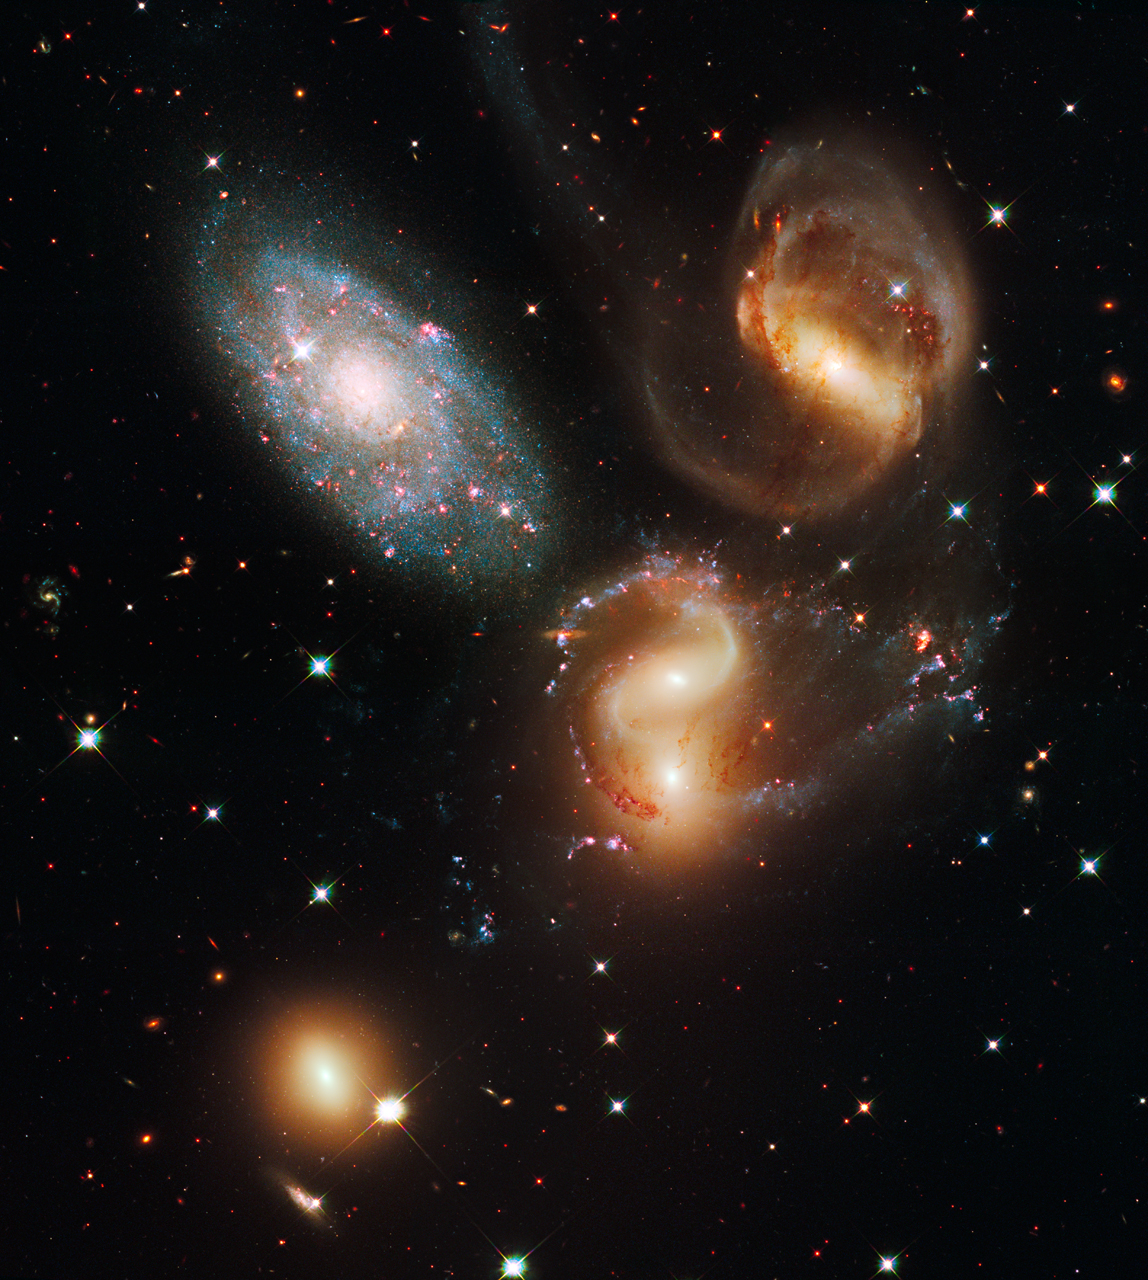
\includegraphics[width=0.7\textwidth]{stephans_quintet.jpg}
  \caption{Hickson compact group 92, known as Stephan's Quintet.
    Image credit: NASA/Hubble Space Telescope.}
  \label{fig:steph_quintet}
\end{figure}

A subclass of galaxy groups are what are known as compact groups.
Compact groups were initially defined by \citet{hickson1982} by the
following criteria:

\begin{itemize}
  \item $N(\Delta m = 3) \ge 4$

  \item $\theta_N \ge 3\,\theta_G$

  \item $\mu_e \le 26.0\,\mathrm{mag}\,\mathrm{arcsec^{-2}}$
\end{itemize}

\noindent
where $N(\Delta m = 3)$ is the number of galaxies within 3 magnitudes
of the brightest galaxy in the group, $\mu_e$ is the effective surface
brightness of the galaxies, $\theta_G$ is the angular diameter of the
smallest circle containing the centres of all group galaxies, and
$\theta_N$ is the angular diameter of the largest circle containing no
galaxies brighter than the surface brightness constraint
\citep{hickson1982, mcconnachie2009}.
\par
Compact groups have proven to be important probes of galaxy evolution,
as due to the close proximity of members many galaxy interactions are
favoured.  When comparing the properties of galaxies in compact groups
to those in loose groups (groups which do not satisfy the Hickson
criteria) it has been shown that galaxies in compact groups tend to be
more evolved.  Namely, they have higher fractions of red, passive,
early-type galaxies as well as older stellar populations and lower
SSFRs \citep{coenda2012, coenda2015}.

\section{The environmental dependence of galaxy properties}
\label{sec:enviro_dependence}

\subsection{Local galaxy density}
\label{sec:local_density}

\subsection{Halo mass}
\label{sec:halo_mass}

\begin{figure}
  \centering
  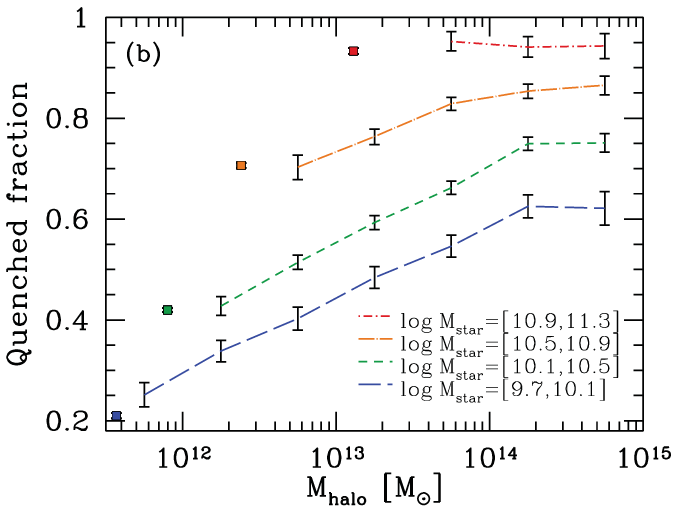
\includegraphics[width=0.8\textwidth]{quenchFrac_wetzel.png}
  \caption{Galaxy quenched fraction ($\mathrm{SSFR} <
    10^{-11}\,\mathrm{yr^{-1}}$) versus halo mass for central galaxies
    (solid points) and satellite galaxies (dashed lines) in bins of stellar mass.  Image credit: \citet{wetzel2012}.}
  \label{fig:quenchFrac_wetzel}
\end{figure}

Across galaxy groups and clusters, a wide range of halo masses is
spanned.  From $\sim\! 10^{12}\Msun$ for low-mass groups, up to
$\gtrsim\! 10^{15}\Msun$ for rich clusters of galaxies.  The
properties of galaxies in these groups and clusters seem to depend on
their host halo mass, although their is still debate as to how strong
of an affect that this is.  For example,
Fig.~\ref{fig:quenchFrac_wetzel}, taken from \citet{wetzel2012}, shows
that galaxies in high-mass haloes tend to have large quenched
fractions, in particular for low-mass galaxies.  Other studies have
also found that color and morphology correlate with halo mass
\citep[e.g.][]{kimm2009, wilman2012}, with galaxies in high mass
haloes tending to be red and early-type.

\subsection{Radial position}
\label{sec:radial_pos}

\begin{figure}
  \centering
  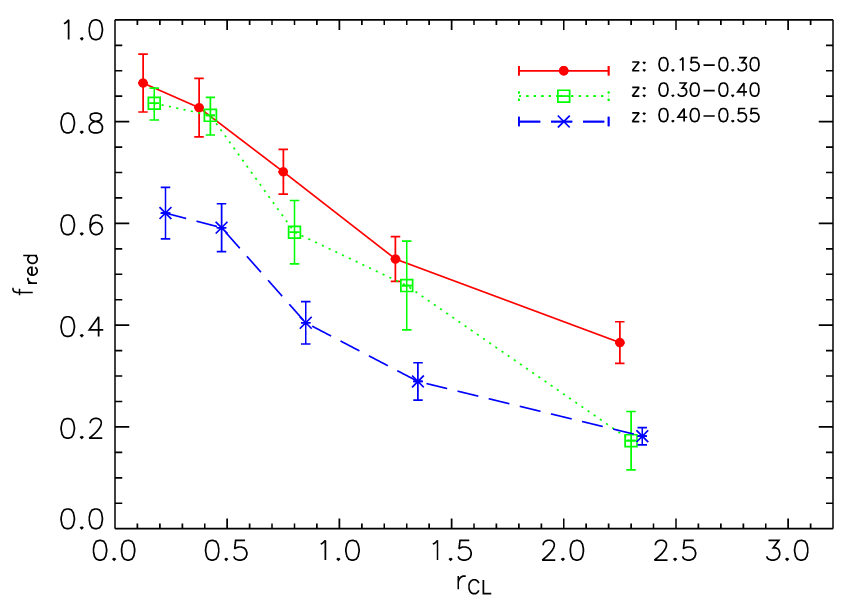
\includegraphics[width=0.8\textwidth]{redFrac_r_li.png}
  \caption{Red fraction versus cluster centric radius for galaxies in
    CNOC clusters.  Colours correspond to three different redshift
    ranges. Image credit: \citet{li2009}.}
  \label{fig:redFrac_r_li}
\end{figure}

On top of correlating with the mass of the host halo, galaxy
properties also show a strong dependence on their group-centric
radius.  Galaxies at small radii near the group centre have been shown
to have red colours \citep{blanton2007b, hansen2009, li2009,
  prescott2011}, reduced star formation
\citep{rasmussen2012, wetzel2012, haines2015}, and earlier type
morphologies
\citep{whitmore1993, goto2003, postman2005, fasano2015}.  Conversely, galaxies in the outer regions of
haloes are preferentially blue, star-forming, with late-type
morphologies.  Fig.~\ref{fig:redFrac_r_li} shows an example from
\citet{li2009} where a clear anti-correlation is seen between red
fraction and cluster-centric radius for galaxies in cluster from the
Canadian Network for Observational Cosmology (CNOC) Survey. In
addition to considering the projected radial
position of a galaxy, recent studies have used velocity-radius phase
space to divide galaxy group and cluster populations into three main
classes: those infalling onto the halo for the first time, those
virialized at small radii, and those ``backsplashing'' beyond the
virial radius after a pericentric passage
\citep[e.g.][]{mahajan2011}.  The
properties of galaxies have been shown to differ based upon which of
these subclasses they are a part of.  For instance, infalling galaxies
have been shown to have enhanced star formation rates \citep{noble2016}, post-starburst galaxies preferentially reside in
intermediate regions of phase space \citep{muzzin2014}, as well
backsplash galaxies should have lower masses due to tidal mass loss
during pericentric passage \citep{gill2005}.  

\subsection{Group dynamical state}
\label{sec:dyn_state}

\begin{figure}[!ht]
  \centering
  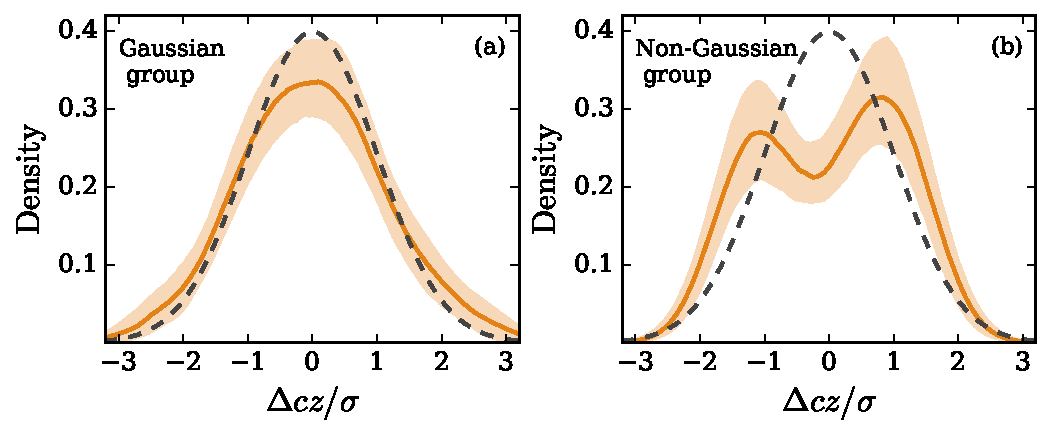
\includegraphics[width=\textwidth]{vdist.pdf}
  \caption{Projected velocity distributions for galaxies in a
    Gaussian (left) and a non-Gaussian (right) SDSS group.  Solid line
    is the median of 1000
  bootstrap resamplings and shaded regions correspond to 68 per cent
  confidence intervals, dashed line corresponds to the standard normal
  distribution.}
  \label{fig:vdist}
\end{figure}

Galaxy groups can be broadly classified by their dynamical states.
Galaxy populations of dynamically old, relaxed groups will show
line of sight velocity distributions which are well fit by a Gaussian
profile, whereas galaxy populations in dynamically young, unrelaxed
groups will have velocity distributions which show stronger deviations
from normality.  The degree to which galaxy properties correlate with
the dynamical state of their host group is still a question of active
research, where no strong concensus has been reached
\citep[e.g.][]{biviano2002, ribeiro2013b}.  Previous studies have
indicated that galaxies in G groups tend to be redder than galaxies in
NG groups \citep{ribeiro2010, carollo2013, ribeiro2013a}.  More
directly investigating star-forming and morphological properties,
\citet{hou2013} find detectable difference between the quiescent
fractions of galaxies in G versus NG groups as a function of
redshift.  More recently, \citet{roberts2016b} have found that
low-mass galaxies in the virialized region of NG groups have enhanced
star-forming and disc fractions compared to galaxies in the same
region of G groups, whereas no differences are detected for infalling
galaxies 

\section{Star formation quenching}
\label{sec:sfr_quench}

It has been well established that populations of galaxies are bimodal
in SFR across essentially all environments (see Fig.~\ref{fig:m_sfr})
\citep[e.g.][]{wetzel2012}, with galaxies either actively forming
stars as
part of the blue cloud or evolving quiescently on the red sequence.  A
question which has had much attention devoted to it is determining
what are the dominant mechanism(s) which are shutting down star
formation in galaxies.  In particular, it has been argued that there
are to main classes of SFR quenching occuring in the Universe: secular
or mass-quenching, and environmental quenching.  The dichotomy between
these two quenching modes is outlined in detail by \citet{peng2010},
where they conclude that low-mass ($\lesssim \! 10^{10.5}\Msun$)
galaxies in the local Universe are quenched by environmental
mechanisms and that galaxies more massive than $\sim \!
10^{10.5}\Msun$ are quenched through internal, secular processes.  

\subsection{Environmental quenching}
\label{sec:enviro_quench}

\noindent \textit{\textbf{Ram pressure stripping}}
\smallskip
\newline
A straight forward way to quench the star formation of a galaxy
is to directly remove the cold gas reserves from the disc.  A commonly invoked
mechanism to achieve this is the ram pressure stripping of cold gas by the
intracluster medium (ICM).  Galaxies will feel a ram pressure force as
they move through the ICM and if this force is enough to overcome to
galaxy's gravitational potential then gas can be stripped from the
disc.  The ram pressure felt by a galaxy scales with the density of
the ICM as well as the square of the galaxy velocity relative to the ICM,
$P_{RP} \propto \rho v^2$ \citep{gunn1972}, and therefore should be
most effective in the cores of high-mass clusters where both densities
and galaxy velocities are high.  One of the characteristic
features of ram pressure stripping is the rapid timescales over which
it is able to quench star formation, if ram pressure stripping is
acting efficiently then cold gas can be removed in $\lesssim
\! 1\,\mathrm{Gyr}$ \citep{abadi1999, quilis2000, roediger2005,
  steinhauser2016}.  Studies which require short
quenching timescales to account for observational results often use
this fact to argue that ram pressure stripping is playing an important
role \citep{muzzin2014, fillingham2015, wetzel2015}.  Additionally, it
is possible to constrain ram
pressure stripping by looking for direct evidence.  For example,
H\textsc{i} distributions which are extended in the direction opposite
to the motion of the galaxy are interpretted as evidence of ram
pressure stripping \citep{kenney2004, chung2007,
  chung2009, kenney2015}.  It is also important to note that while
ram pressure stripping appears to have a measureable affect on atomic
hydrogen (at least in high-mass clusters), how
effectively it can remove molecular hydrogen from the disc is still a
debated question \citep{boselli2002, boselli2006, fumagalli2009,
  sivanandam2014} \newline

\noindent \textit{\textbf{Starvation}}
\smallskip
\newline
As opposed to the removal of cold gas from the disc, starvation (also
sometimes referred to as ``strangulation'') is the prevention of the
replenishment of cold gas reserves.  This can occur either through the
stripping of hot halo gas, or by preventing the hot halo gas from
cooling and accreting onto the galactic disc.  \citet{larson1980}
first proposed that preventing spiral galaxies from accreting new gas
could account for the high fractions of passive S0 galaxies observed
in local clusters.  Compared to ram pressure stripping, quenching by
starvation will occur over much longer timescales on the order of
$\sim 2 - 
10\,\mathrm{Gyr}$ \citep{wheeler2014, fillingham2015, peng2015,
  wetzel2015}.  The precise quenching time
will be set by the gas consumption timescale of a given galaxy, as
once a galaxy it cut-off from gas accretion it will only form stars
until it has exhausted its existing cold-gas reserves.  The results of
previous works have indicated that in many cases long quenching times
are required to reproduce observational results \citep{balogh2000,
  balogh2000b, wetzel2013, wheeler2014}, which tends to be interpretted as
evidence for the importance of starvation as a quenching mechanism.
Recently \citet{peng2015} have presented a novel technique for
observationally constraining the importance of starvation.  Peng et
al. propose that evidence for starvation can be gleaned through
examining the stellar metallicities for galaxies.  If a galaxy is
quenched via starvation then its stellar metallicity should continue
to rise as it exhausts its existing cold-gas reserves, therefore the
population of passive galaxies should show higher metallicites than
the population of star-forming galaxies.  Peng et al. argue that this
serves as a method to distinguish between starvation and ram pressure
stripping, as due to the rapid nature of ram pressure stripping, the
metallicity difference between star-forming and passive galaxies would
not be expected.\newline  

\noindent \textit{\textbf{Galaxy interactions}}
\smallskip
\newline
As opposed to quenching through interactions with surrounding gas, it
is possible that quenching can be driven by more direct interactions
between galaxies.  These interactions can be broadly divided into
three main categories: major mergers, minor mergers, and impulsive
interactions.  Major mergers (mass ratio, $M_1/M_2 \lesssim 3-4$) have
been shown to induce starburst events which can very quickly exhaust the gas
reserves of a galaxy, leaving it quenched \citep[e.g.][]{mihos1994b}.
As well, observations of closly paired galaxies show that paired
galaxies of similar mass demonstrate stong enhancements in SFRs with
decreasing seperation, consistent with interaction induced starbursts
\citep{ellison2008, davies2015}.  Minor mergers ($M_1/M_2 \gtrsim
3-4$) have also been shown to be capable of inducing starbursts in the
primary galaxy \citep[e.g.][]{mihos1994a}, and seeing as minor mergers
are significantly more common than major mergers \citep{lotz2011},
this plays a potentially important role in transforming galaxies.
Observations of galaxies in minor pair haves shown that star formation
in enhanced in the higher mass primary, but suppressed in the
secondary galaxy \citep{davies2015}.  As opposed to galaxy mergers,
impulsive interactions are high-speed close encounters between
galaxies, also referred to as ``galaxy harassment'' \citep{moore1996}.
Like galaxy mergers, harassment is capable of inducing bursty star
formation as multiple high-speed encounters can funnel cold gas to the
central regions of galaxies and therefore fuel intense star formation
\citep{fujita1998}.  

\subsection{Mass Quenching}
\label{mass_quench}

While low-mass galaxies tend to be quenched via environmental
mechanisms, high-mass galaxies seem to be preferentially quenched
through secular processes.  The most commonly invoked source of mass
quenching is the feedback from Active Galactic Nuclei (AGN).  Jets and
galactic scale winds from AGN can not only displace cold gas from the
galactic disc, but also heat surrounding gas to prevent cooling and
subsequent star formation.  Semi-analytic models as well as
hydrodynamic simulations with subgrid AGN prescriptions have shown
that AGN feedback can significantly suppress star formation and
therefore more closly match observations, in
particular within high-mass galaxies \citep[e.g.][]{somerville2008,
  dubois2013, bongiorno2016}

% Bibliography
%
\bibliographystyle{apj}
\bibliography{masters-thesis}
